\documentclass[11pt,a4paper]{article}

\usepackage[nohyperref]{acl2018} % references acl2018.sty
\usepackage{times}
\usepackage{latexsym}
\usepackage{multirow}
\usepackage{graphicx}
\usepackage{pdflscape}
\usepackage{url}

\aclfinalcopy % Uncomment this line to show the author and remove the line numbers on the sides

\newcommand{\tabitem}{~~\llap{\textbullet}~~}
\newcommand\BibTeX{B{\sc ib}\TeX}

\title{Final Project Report - BETTER TITLE NEEDED}

\author{Carmen Easterwood \\
  W266 Natural Language Processing with Deep Learning \\
  Summer 2018 \\
}

\date{August 10, 2018}

%%%%%%%%%%%%%%%
% End header information
%%%%%%%%%%%%%%%

\graphicspath{ {../../plots/} }

\begin{document}
\maketitle

\begin{abstract}
In this paper, I develop a topic classification model for news articles. I test multiple different model inputs, but find that feeding the full article text into the model still generates the best results. The highest performing model (so far) is a logistic regression model with accuracy of 77\%, and F1 scores to be calculated for the final paper.
\end{abstract}

\section{Introduction}
\label{sec:intro}

Classifying news articles by topic is an important form of content analysis. It lets us know what journalists are writing about, whether that is changing over time, and the relative important of different topics. Tagging articles by topic also makes article searches more efficient for news consumers and researchers. However, manual topic-coding is quite time-consuming, so automating this process can save time and money for news organizations. This paper will develop a supervised topic classification model using New York Times news articles.

\section{Background}
\label{sec:back}

There is a large literature looking at various aspects of document classification, but only a few have focused on evaluating newspaper articles. Martin and Johnson (2015) used a dataset from the San Jose Mercury News and found that using a nouns-only or lemmatized version of the articles improved topic classification. However, theirs was an unsupervised model, so they evaluated their model using techniques that are not applicable in a supervised setting.

Meanwhile, Wermter and Hung (2002) created a semi-supervised self-organizing memory (SOM) model for topic generation of Reuters news articles. They used WordNet relationships to assist their model and thus limited their model input to only the nouns and verbs found in WordNet. This allowed them to achieve accuracies over 95\%, but generalizability may be limited due to this use of WordNet.

Other recent papers have looked at supervised topic classification for non-news documents. Karan et al (2016) looks at classification of Croatian political texts) using word2vec, logistic regression, Gaussian NB, and gradient-boosted trees, as well as a couple of postprocessing rules, to reach an F1 score of 77\% for major topics. Glava� et al (2017) looks at SVM and CNN models for multiple languages, and for monolingual English models finds that CNNs perform best with an accuracy of 57\%. In this paper, I will test whether some of the ideas and techniques used for classification of non-news documents can be successfully extended to the news article setting.


\section{Methods}
\label{sec:methods}

\subsection{Dataset}
\label{ssec:dataset}

I used the New York Times Annotated Corpus, which contains 1.8 million articles from 1987-2007, labeled with topics, subtopics, and newspaper sections. Due to computing power limitations, I have selected a random sample of 10,000 articles to parse and use as data for the model. The articles are randomly split so that approximately 75\% are training data, 5\% are development data, and 20\% test data.

\subsection{Model Input}
\label{ssec:input}

Based on my review of the literature, I tested five different model inputs, some of which are specific to the newspaper context. Table~\ref{tbl:inputs} shows some key statistics for each type of model input for my random sample of 10,000 articles.

\begin{enumerate}
\item Full text of article
\item Nouns-only version of the full text \cite{Martin:15}
\item Lemmatized version of the full text \cite{Martin:15}
\item Article's headline \cite{Wermter:02}
\item Article's lead paragraph, which is supposed to hook the reader, and in a news context often summarizes important details of the story \cite{NPR}
\end{enumerate}

\begin{table}
	\centering
	\small
	%\makebox[\linewidth]{
	\begin{tabular}{| l | r r r | r r r |}
		\hline
		\multirow{2}{*}{\textbf{Model Input}} & \multicolumn{3}{c|}{\textbf{Training Words}} & \multicolumn{3}{c|}{\textbf{Training Vocab (Unique Words)}} \\
		\cline{2-7}
		& \textbf{Count} & \textbf{\% Full Text} & \textbf{Avg. per Article} & \textbf{Count} & \textbf{\% Full Text} & \textbf{Avg. per Article} \\
		\hline
		Full Text & 5,033,755 & 100 & 684 & 87,541 & 100 & 264 \\
		Lead Paragraph & 740,321 & 15 & 103 & 40,309 & 46 & 61 \\
		Headlines	& 57,752 & 1 & 8 & 11,150 & 13 & 6 \\
		Nouns Only & 1,371,922 & 27 & 184 & 65,029 & 74 & 112 \\
		Lemmatized & 5,120,323 & 102 & 686 & 76,109 & 87 & 246 \\
		\hline
	\end{tabular}
	%}
	\caption{Model Inputs}
	\label{tbl:inputs}
\end{table}

\subsection{Model Output}
\label{ssec:output}

The NYT dataset has multiple ways of classifying articles. Table~\ref{tbl:output} shows examples of the four different ways that six articles were classified. In my models I use the \texttt{desk} column as my model output variable because:

\begin{enumerate}
\item It has the lowest percentage of null values
\item It never assigns multiple descriptions to the same article
\end{enumerate}

\begin{table}
\centering
\footnotesize
%\makebox[\linewidth]{
\begin{tabular}{| l | l | l | l |}
	\hline
	\textbf{Desk} & \textbf{General Descriptor} & \textbf{Online Sections} & \textbf{Taxonomic Classifier} \\
	\hline
	Foreign Desk & \tabitem Immigration and Refugees & \tabitem World & \tabitem Top/News/World/Europe \\
	& \tabitem Jews & & \tabitem Top/News/World/Countries and Territories/Austria \\
	& \tabitem Music & & \tabitem Top/Features/Arts/Music \\
	& \tabitem Religion and Churches & & \tabitem Etc. (8 others) \\
	\hline
	Book Review Desk & \tabitem Books and Literature & \tabitem Arts & \tabitem Top/Feature/Arts \\
	& & \tabitem Books & \tabitem Top/Features/Books \\
	& & & \tabitem Top/Features/Books/Book Reviews \\
	\hline
	Classified & & \tabitem Paid Death Notices & \tabitem Top/Classifieds/Paid Death Notices \\
	\hline
\end{tabular}
%}
\caption{Possible Model Outputs}
\label{tbl:output}
\end{table}

However, \texttt{desk} still requires some clean-up before use due to misspellings and possible changes to the desk names over time. Table~\ref{tbl:label-clean} shows some examples of how I cleaned the \texttt{desk} variable so the model would have a standardized set of output labels for the articles.

\begin{table}
\centering
\small
\begin{tabular}{llr}
	\hline
	\textbf{Cleaned Label Name} & \textbf{Original Label Name} & \textbf{Articles} \\
	\hline
	book review & Book Review Desk & 176 \\
	\hline
	\multirow{9}{*}{business \& financial} & Business World Magazine & 1 \\
	& Business/Finance Desk & 1 \\
	& Business/Financial Desk & 628 \\
	& Business\textbackslash Financial Desk & 1 \\
	& E-Commerce & 1 \\
	& Financial Desk & 1106 \\
	& Financial Desk; & 2 \\
	& Money and Business/Financial Desk & 79 \\
	& SundayBusiness & 14 \\
	\hline
	\multirow{2}{*}{cars} & Automobiles & 9 \\
	& Cars & 4 \\
	\hline
\end{tabular}
\caption{Label Cleaning Examples}
\label{tbl:label-clean}
\end{table}

After cleaning, roughly 95\% of articles fall into the top 20 categories, and then there are a large number of very small categories with just a couple of articles. I therefore created an \texttt{<OTHER>} category as a catchall for these tiny categories, which individually don't have enough data for a model to learn very well. Figure~\ref{fig:topnhist} shows the frequency distribution of the top 20 category labels, plus \texttt{<OTHER>}.

\begin{figure}
\centering
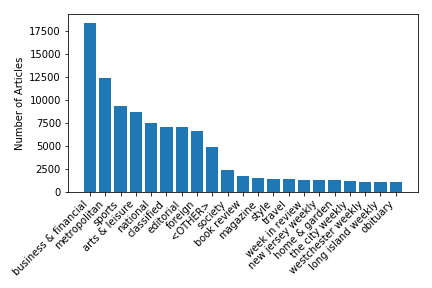
\includegraphics[scale=0.6]{top_n_labels_histogram}
\caption{Frequency of Top 20 Labels + \small{\tt <OTHER>}}
\label{fig:topnhist}
\end{figure}

\subsection{Models}
\label{sec:models}

% For each set of training data, I TF-IDF vectorize it before feeding it into models.

I used multinomial na\"{i}ve Bayes and multi-class logistic regression (one vs. rest) as simple baseline models. I will also be testing more complicated models based on my review of some relevant literature (SVM, CNN, and gradient boosted trees).

\cite{Glavas:17} -- 
\citep{Glavas:17} -- 
\citet{Glavas:17} -- 
\citealp{Glavas:17} -- 
\citeyearpar{Glavas:17} -- 
\citeauthor{Glavas:17} -- 
\shortcite{Glavas:17} -- 
\cite{Glavas:17,Wermter:02}

\cite{Karan:16}

\cite{Martin:15}

\cite{GloVe}

\begin{quote}
``Stuff ... ''
\end{quote}

\section{Results \& Discussion}
\label{sec:results}

Note: \cite{Wermter:02} uses only top 8 topics.

\begin{table}
\centering
\small
\begin{tabular}{|l|rrr|p{1.2cm}|}
	\hline
	\multirow{2}{*}{\textbf{Model Input}} & \multicolumn{3}{c|}{\textbf{Model Type}} & \multicolumn{1}{c|}{\textbf{Best}} \\
	\cline{2-4}
	& \textbf{LR} & \textbf{MNB} & \textbf{NN} & \multicolumn{1}{c|}{\textbf{Model}} \\
	\hline
	Full Text & 0. & 0. & 0. & \\
	Lead Paragraph & 0. & 0. & 0. & \\
	Headlines & 0. & 0. & 0. & \\
	Nouns & 0. & 0. & 0. & \\
	Lemmas & 0. & 0. & 0. & \\
	\hline
	\textbf{Best Input} & & & & \textbf{-} \\
	\hline
\end{tabular}
\caption{Model Accuracies}
\label{tbl:acc}
\end{table}

\section{Conclusion}
\label{sec:conc}

An interesting future project would be to run an unsupervised topic classification algorithm on this corpus (e.g. \citeauthor{Martin:15}~\shortcite{Martin:15} use the Latent Dirichlet Allocation algorithm) and compare those results to the supervised learning results.

\bibliography{final-report} % references .bib file
\bibliographystyle{acl_natbib} % references acl_natbib.bst

\end{document}
